\documentclass[12pt]{article}
\usepackage[utf8]{inputenc}
\usepackage[brazilian]{babel}
\usepackage{graphicx}
\usepackage{amsmath}
\usepackage{hyperref}
\usepackage{geometry}
\usepackage{listings}
\usepackage{xcolor}
\usepackage{subcaption}

\geometry{margin=1in}

\definecolor{codegreen}{rgb}{0,0.6,0}
\definecolor{codegray}{rgb}{0.5,0.5,0.5}
\definecolor{codepurple}{rgb}{0.58,0,0.82}
\definecolor{backcolour}{rgb}{0.95,0.95,0.92}

\lstdefinestyle{mystyle}{
    backgroundcolor=\color{backcolour},   
    commentstyle=\color{codegreen},
    keywordstyle=\color{magenta},
    numberstyle=\tiny\color{codegray},
    stringstyle=\color{codepurple},
    basicstyle=\ttfamily\footnotesize,
    breakatwhitespace=false,         
    breaklines=true,                 
    captionpos=b,                    
    keepspaces=true,                 
    numbers=left,                    
    numbersep=5pt,                  
    showspaces=false,                
    showstringspaces=false,
    showtabs=false,                  
    tabsize=2
}

\lstset{style=mystyle}

\title{Criação e Identificação de Processos em Linux}
\author{Sistemas Operacionais}
\date{\today}

\begin{document}

\maketitle

\section{Introdução}

Este relatório investiga o comportamento da criação de processos em Linux, com foco no funcionamento das funções \texttt{getpid()}, \texttt{getppid()} e \texttt{fork()}. Foi desenvolvido um programa em C que cria uma hierarquia de processos (pai, filho e neto) com diferentes configurações de tempo de espera para observar como o sistema gerencia os identificadores de processos (PIDs) e as relações entre processos.

\section{Análise do Programa}

O programa implementa três experimentos distintos para demonstrar diferentes aspectos do gerenciamento de processos:

\begin{itemize}
    \item \textbf{Experimento A}: "Sem espera" - Nem o filho nem o neto dormem
    \item \textbf{Experimento B}: "Pai espera" - O processo filho dorme por 100 microssegundos
    \item \textbf{Experimento C}: "Neto órfãos" - O processo neto dorme por 100 microssegundos
\end{itemize}

Cada experimento é executado múltiplas vezes (o experimento A é repetido 10 vezes, enquanto B e C são repetidos 5 vezes cada), e o programa inteiro é executado em 3 iterações.

\subsection{Estrutura do Código}

O programa utiliza a função \texttt{fork()} para criar novos processos. A estrutura básica envolve:

\begin{lstlisting}[language=C]
// Criacao do processo filho
pid_t child_pid = fork();
switch (check_fork(child_pid)) {
    case FORK_CHILD:
        // Código executado pelo filho
        
        // Criação do processo neto
        pid_t grand_child_pid = fork();
        switch (check_fork(grand_child_pid)) {
            case FORK_CHILD:
                // Codigo do neto
                break;
            case FORK_PARENT:
                // Codigo do filho apos criar o neto
                break;
        }
        exit(0); // Filho termina
        break;
        
    case FORK_PARENT:
        // Codigo do processo pai
        break;
}
\end{lstlisting}

O programa registra o PID e PPID de cada processo em momentos especificos e os processos filho e neto podem dormir por um tempo determinado de acordo com o experimento.

\section{Análise dos Resultados}

Vamos analisar os resultados dos experimentos para entender o comportamento dos processos no sistema Linux.

\subsection{Diferenças entre PIDs}

\begin{figure}[h]
    \centering
    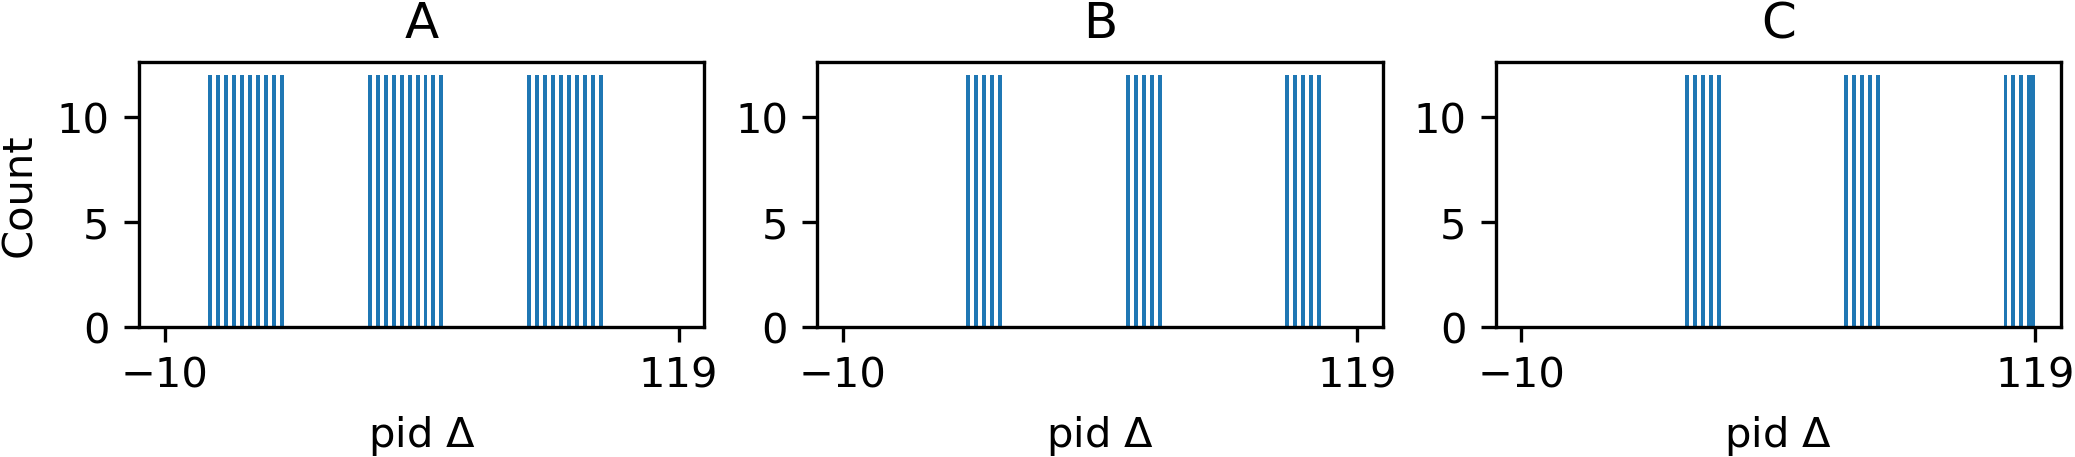
\includegraphics[width=0.8\textwidth]{figures/delta_histogram.png}
    \caption{Histograma da diferenca entre PIDs de processos filhos e seus pais}
    \label{fig:delta_histogram}
\end{figure}

A Figura \ref{fig:delta_histogram} mostra a distribuicao das diferencas entre os PIDs dos processos filhos e seus pais. Podemos observar que em geral os PIDs sao atribuidos de forma sequencial, com diferencas pequenas entre processos pai e filho. Isso e um comportamento esperado do escalonador do Linux, que tende a atribuir PIDs consecutivos quando os processos sao criados em sequencia rapida.

\begin{figure}[h]
    \centering
    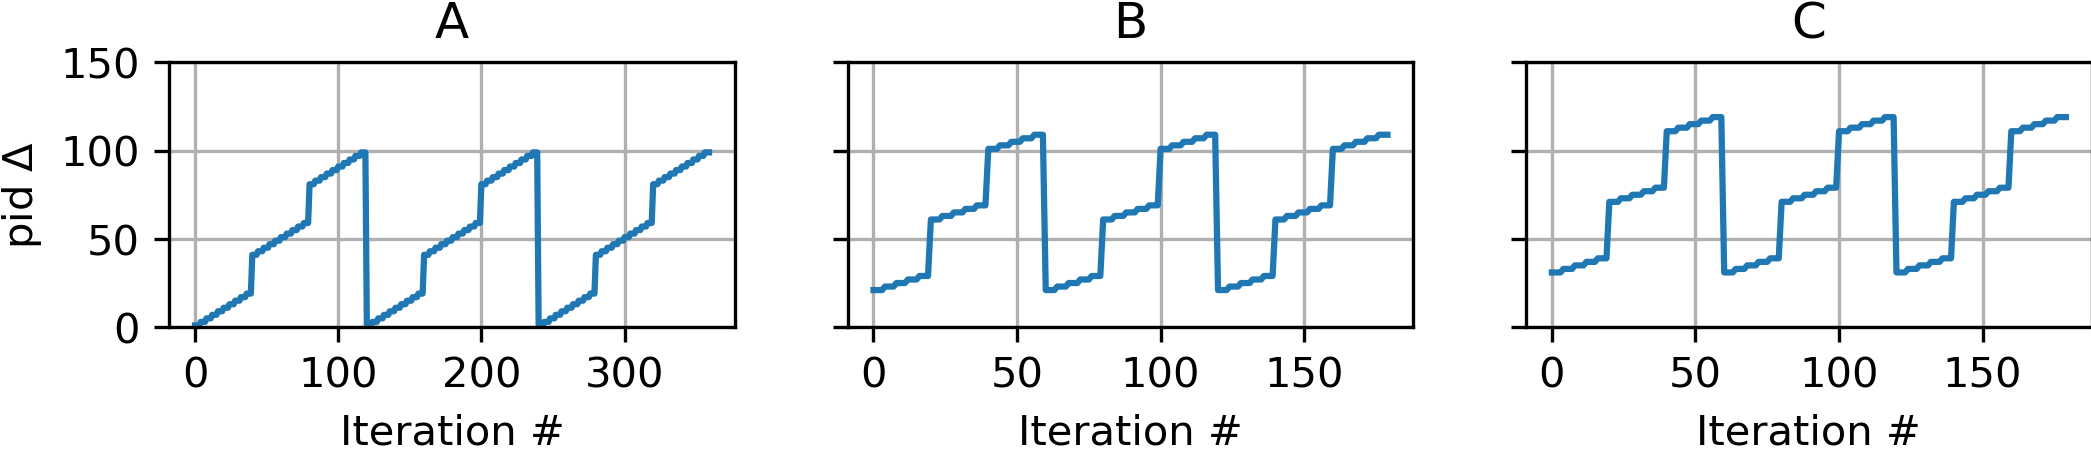
\includegraphics[width=0.8\textwidth]{figures/delta_iteration.png}
    \caption{Variacao da diferenca de PIDs ao longo das iteracoes}
    \label{fig:delta_iteration}
\end{figure}

A Figura \ref{fig:delta_iteration} mostra como essa diferenca varia ao longo das iteracoes. Percebemos que ha um padrao consistente nas atribuicoes de PIDs, com mudancas graduais nas diferencas. Isso confirma que o kernel Linux mantem um contador global de PIDs e o incrementa a medida que novos processos sao criados.

\subsection{Processos Órfãos}

\begin{figure}[h]
    \centering
    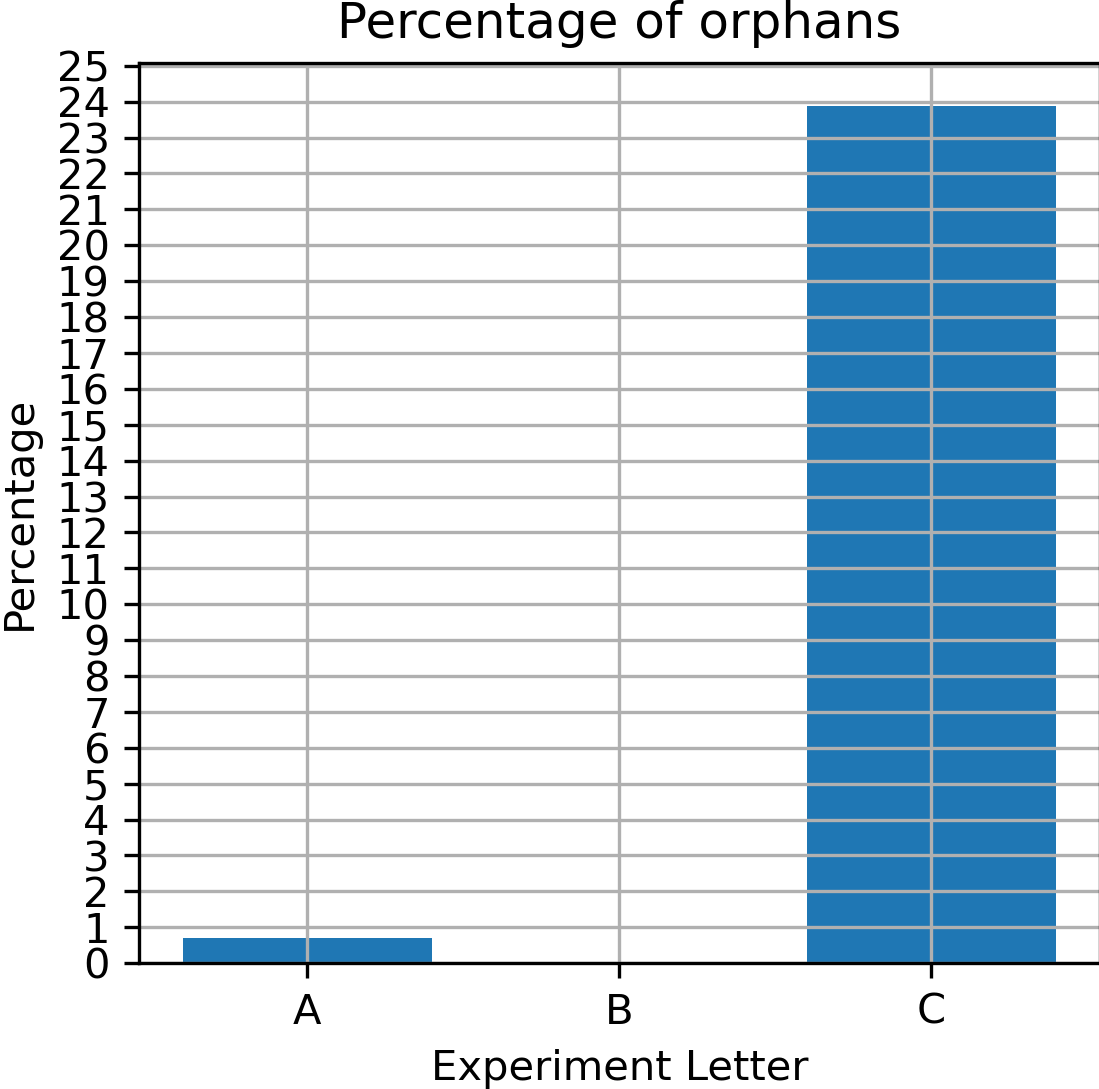
\includegraphics[width=0.5\textwidth]{figures/orphans.png}
    \caption{Porcentagem de processos orfaos por experimento}
    \label{fig:orphans}
\end{figure}

A Figura \ref{fig:orphans} demonstra um resultado fundamental: no Experimento C, onde os processos netos dormem por 100 microssegundos, ha um percentual significativamente maior de processos orfaos (com PPID=1). Isso acontece porque:

\begin{enumerate}
    \item O processo filho cria o neto
    \item O neto dorme por 100 microssegundos
    \item O filho termina sua execução antes do neto acordar
    \item O neto, ao acordar, torna-se orfao e e "adotado" pelo processo init (PID 1)
\end{enumerate}

Este comportamento e parte do mecanismo do Linux para evitar processos zumbis e garantir que todos os processos tenham um pai valido.

\section{Respostas às Perguntas}

\subsection{Diferenca entre getpid() e getppid()}

A funcao \texttt{getpid()} retorna o identificador de processo (PID) do processo que a chamou, enquanto \texttt{getppid()} retorna o identificador do processo pai (PPID). Esses identificadores sao essenciais para o sistema operacional gerenciar a hierarquia de processos:

\begin{itemize}
    \item O PID e um numero unico atribuido a cada processo no sistema, usado para identificar e controlar o processo.
    \item O PPID indica qual processo criou o processo atual, estabelecendo a relacao pai-filho na hierarquia de processos.
\end{itemize}

\subsection{O que acontece com o PID do processo filho após o fork()}

Apos a execucao do \texttt{fork()}, sao criados dois processos quase identicos: o processo pai original e um novo processo filho. Cada um recebe um tratamento diferente:

\begin{itemize}
    \item O processo filho recebe um novo PID (geralmente o proximo disponivel no contador de PIDs do sistema).
    \item O PPID do processo filho e configurado como o PID do processo pai.
    \item O processo pai mantem seu PID original.
\end{itemize}

Nossos experimentos mostram que os PIDs tendem a ser atribuidos sequencialmente, embora isso nao seja garantido. A diferenca entre o PID do filho e do pai geralmente e pequena quando os processos sao criados rapidamente em sequencia.

\subsection{Como o sistema operacional identifica e organiza os processos}

O Linux usa uma estrutura de dados chamada \texttt{task\_struct} para representar cada processo. Cada instancia desta estrutura contem:

\begin{itemize}
    \item Um identificador único (PID)
    \item Referencia ao processo pai (PPID)
    \item Informacoes sobre recursos alocados
    \item Estado do processo
    \item Informacoes de escalonamento
\end{itemize}

Os processos sao organizados em uma hierarquia em arvore, onde cada processo (exceto o init com PID 1) tem um pai. Quando um processo pai termina antes de seus filhos, o sistema reatribui esses filhos ao processo init (PID 1), tornando-os "orfaos", como vimos claramente no Experimento C.

\subsection{Previsao do numero de mensagens apos o fork()}

Nao e possivel prever com certeza absoluta o numero exato de mensagens impressas apos um \texttt{fork()}, pois isso depende de varios fatores:

\begin{itemize}
    \item Escalonamento de processos pelo sistema operacional
    \item Temporizacao entre a execucao de processos pai e filho
    \item Condicoes do sistema no momento da execucao
\end{itemize}

No nosso programa, cada chamada de \texttt{fork()} duplica o fluxo de execucao. Com dois \texttt{fork()} em cascata, temos teoricamente ate 4 caminhos de execucao. Porem, como o codigo usa \texttt{switch} para diferenciar comportamentos entre pai e filho, o numero de mensagens e controlado mais precisamente.

\subsection{Por que o mesmo programa pode ter multiplos processos com identidades distintas}

O mesmo programa pode ter multiplos processos com identidades distintas devido a natureza da chamada \texttt{fork()}, que:

\begin{itemize}
    \item Cria uma copia quase identica do processo chamador (incluindo codigo, dados, heap e pilha)
    \item Atribui um novo PID ao processo filho
    \item Permite que os processos sigam caminhos de execucao diferentes apos o \texttt{fork()}
\end{itemize}

Isso e fundamental para o modelo de concorrencia do Unix/Linux, permitindo que um unico programa execute multiplas tarefas paralelamente com isolamento adequado entre processos. No nosso experimento, isso e evidenciado pelos diferentes comportamentos dos processos pai, filho e neto, cada um com seu proprio PID e comportamento especifico.

\section{Conclusão}

Os experimentos realizados demonstram claramente como o Linux gerencia a hierarquia de processos e os identificadores de processos. Observamos:

\begin{itemize}
    \item A atribuicao sequencial de PIDs
    \item O impacto do tempo de execucao na criacao de processos orfaos
    \item Como os mecanismos de \texttt{fork()} permitem criar hierarquias de processos
\end{itemize}

O comportamento do sistema operacional ao lidar com processos orfaos (reatribuindo-os ao processo init) e especialmente relevante para evitar processos zumbis e manter a integridade da hierarquia de processos. Estes conceitos sao fundamentais nao apenas para a programacao de sistemas, mas tambem para a compreensao da arquitetura de sistemas operacionais modernos.

\end{document}